\documentclass[12pt, a4paper]{article}
\renewcommand*\contentsname{Inhaltsverzeichnis}
\usepackage[ngerman]{babel}
\usepackage{mathptmx}
\usepackage{blindtext}
\usepackage{emptypage}
\usepackage{wrapfig}
\usepackage[pdftex]{graphicx}
\usepackage{geometry}
\usepackage{setspace}
\usepackage[version=4,arrows=pgf-filled,
textfontname=sffamily,
mathfontname=mathsf]{mhchem}
\usepackage{hyperref}
\usepackage{multirow}
\usepackage{mathcomp}
\usepackage[table]{xcolor}
\usepackage{array}
\usepackage{csquotes}
\usepackage[backend=biber,style=chem-acs,sorting=none]{biblatex}
\addbibresource{literatur.bib}  % Deine .bib-Datei einbinden

\DeclareCiteCommand{\cite}
  {\usebibmacro{prenote}}
  {\textsuperscript{\printfield{labelnumber}}}
  {\multicitedelim}
  {\usebibmacro{postnote}}


 \geometry{
 a4paper,
 total={170mm,257mm},
 left=25mm,
 top=25mm,
 }
\setstretch{1.213}


\newcommand{\datum}{\day.\month.\year}
\DeclareGraphicsExtensions{.pdf,.jpeg,.png,.jpg} 

\begin{document}


\begin{figure}
    \includegraphics[scale=0.14]{Universität_Bayreuth.svg.png}
\end{figure}


%Deckblatt

{\raggedright Universität Bayreuth\\  95447 Bayreuth}


\vspace{5cm}

\begin{center}
{\LARGE\bf{Anorganische Chemie III}} \\  
\vspace{1cm}
{\Large\bf{Hochtemperatur-Supraleiter}}\\
\vspace{0.5cm}
{\large Justus Friedrich\\}
{Studiengang: B.Sc. Chemie\\}
{4. Fachsemester}
\end{center}





\thispagestyle{empty}
\begin{center}
{\small Matrikelnummer: 1956010 \\
E–Mail:  bt725206@myubt.de}
\end{center}

\vspace{5cm}

\begin{center}
  \today
\end{center}


\newpage
%Inhaltsverzeichnis
\tableofcontents
\thispagestyle{empty}


%Teil 1
\newpage
\setcounter{page}{1}
\section{Einleitung}



\subsection{Einführung}
{Supraleiter sind in der heutigen Gesellschaft sehr relevant, vom Large Hadron Collider am Cern über NMR-Geräten bis zum MRT. 
In all diesen Geräten sind Supraleitende Stoffe verbaut, um ein starkes Magnetfeld zu erzeugen. Allerdings ist das mit einem hohen 
Energieaufwand verbunden, da in diesen in der Regel mit Supraleiter verbaut werden, die flüssiges Helium zur Kühlung 
benötigen. Es gibt allerdings auch Hochtemperatur-Supraleiter, die nur flüssigen Stickstoff zur Kühlung benötigen. Allerdings sind die 
meisten der Hochtemperatur-Supraleiter noch nicht Markreif.\cite{Buckel.2013}
}

\subsection{Ziel des Versuchs}
{In dem Versuch soll der Supraleiter $YBa_2Cu_3O_{6-7}$ hergestellt, wobei möglichst viel Sauerstoff eingelagert werden sollte. Anschließend soll die Struktur mittls eines Pulverdiffraktogramms untersucht werden, 
und als Nachweis des Supraleiters auf den Meißner-Ochsenfeld-Effekt untersucht werden.\cite{Skript}
}

\newpage
%Teil2
\section{Durchführung}
\subsection{\texorpdfstring{Synthese von $YBa_2Cu_3O_{6-7}$}{Synthese von YBa2Cu3O6-7}}
{

Dieser Versuch wird durchgehend im Abzug durchgeführt, da Stickoxide entstehen können.
$300.1\ mg$ (1.33 mmol) $Y_2O_5$ wird mit 634.1 mg (7.971 mmol) $CuO$ in ca. 7 mL konzentrierter $HNO_3$. Diese Lösung wird bei ca. 90 °C auf einer 
Rührplatte stark eingeengt. Daraufhin wird mit 30 mL Wasser verdünnt und mit 1.39 g (5.314 mmol) $Ba(NO_3)_2$ versetzt. Danach wird die Lösung wieder eingeengt und mit 
9 mL (160.9 mmol) Ethylenglykol und 4.5 g (23.42 mmol) Zitronensäure versetzt. Daraufhin wird die Lösung so lange eingeengt, bis eine dickflüssige Lösung entstanden ist. 
Dabei kann es zum Aufschäumen und Stickoxid Bildung kommen. Nachdem die Lösung dickflüssig geworden ist, wird sie in einen Tiegel überführt und über einen Bunsenbrenner erhitzt. 
Dabei kann es wieder zum Überschäumen kommen. Wenn keine Dämpfe mehr entstehen wird noch für 10 weitere Minuten mit dem Bunsenbrenner erhitzt. Daraufhin wird das entsandende Pulver für 10 h bei 920 °C getempert. 
Danach wird eine Tablette gepresst und erneut für 8h für 920 °C getempert. Anschließend wird bei 450 °C für 8h in einer $O_2$-angereicherten Atmosphäre getempert.\cite{Skript}
}
\subsection{Charakterisierung}
{
Es wird ein kleines Stück der Tablette abgebrochen und davon ein Pulverdiffraktogramm aufgenommen. Die restliche Tablette wird mit flüssigen Stickstoff gekühlt und vorsichtig auf 
ein Magneten gegeben. 
}



\newpage
\section{Auswertung}
\subsection{Phasenanalyse}
Es wird zunächst über eine XRD-Messung die Phasen bestimmt, die im Supraleiter vorliegen. Das XRD wird in Abbildung \ref{xrdsupraleiter} dargestellt.

\begin{figure}[!h]
  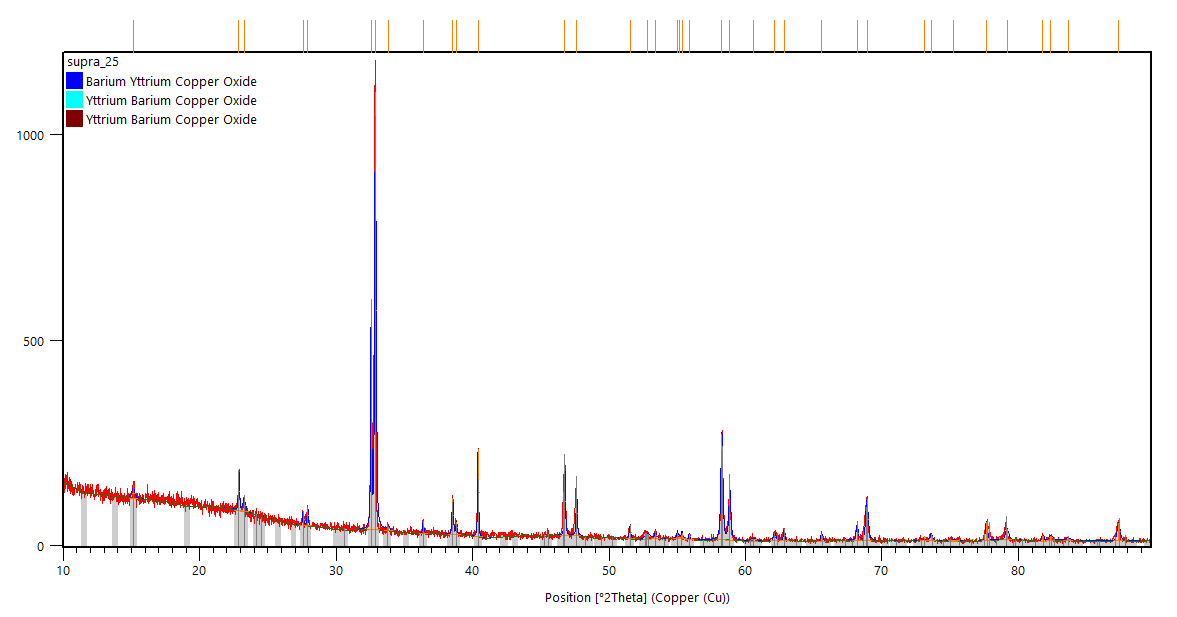
\includegraphics[width=\linewidth]{Supraleiter.png}
  \caption{Dargestellt sind die gemessenen Reflexe der hergestellten Probe \ce{YBa2Cu3O_{7-\delta}}. Zum Vergleich sind die Referenzreflexe von \ce{YBa2Cu3O_{6.54}} (Referenzcode 01-078-1974) mit angegeben.}
  \label{xrdsupraleiter}
\end{figure}

\noindent
Der hergestellte Supraleiter ist Phasenrein. \textit{HighScore Plus} ist sich nur unsicher, wie viel Sauerstoff eingelagert ist. Dabei sind die vorgefunden Oxidationsgraden in Tabelle \ref{Referenzcodesssss} dargestellt.

\begin{table}[!h]
  \caption{Zeigt die gefundnen Oxidationsgraden mit Referenzcodes, \textit{HighScore Plus} Score und Elementarzellenvolumen.}
  \centering
  \begin{tabular}{|>{\centering\arraybackslash}p{0.22\linewidth}|>{\centering\arraybackslash}p{0.22\linewidth}|>{\centering\arraybackslash}p{0.22\linewidth}|>{\centering\arraybackslash}p{0.22\linewidth}|}
    \hline
    \rowcolor{lightgray}
    Oxidationsgrad & Referenzcode & Score & Elementarzellen-Volumen \\
    \hline
    \ce{YBa2Cu3O_{6.50}}&01-082-1603& 43 & 173.855\\
    \hline
    \ce{YBa2Cu3O_{6.54}}&01-078-1974& 78 & 172.95\\
    \hline
    \ce{YBa2Cu3O_{6.8}}&01-080-0491& 75 & 173.16\\
    \hline
    \ce{YBa2Cu3O_{6.84}}&01-080-05071& 32 & 174.10\\
    \hline
    \ce{YBa2Cu3O_{6.948}}&01-080-1969& 60 & 172.38\\
    \hline
  
  \end{tabular}
  \label{Referenzcodesssss}
\end{table}

\noindent
Da bei den Oxidationsgrad \ce{YBa2Cu3O_{6.54}} die höchste Übereinstimmung vorliegt, wird der Zellparameter mit diesem verglichen. Dies wird in Tabelle \ref{KastenlängeferroYBaCuO} dargestellt.
\newpage
\begin{table}[h!]
\caption{\textit{Zeigt die Theoretische und Festgestellte Einheitszelle von den hergestellten \ce{YBa2Cu3O7-\delta} (Referenzcode 01-078-1974). Die Verfeinerung wurde mithilfe des Programmes HighScore Plus durchgeführt. }}
\begin{center}
\begin{tabular}{|>{\columncolor{lightgray}}p{4cm}|>{\centering\arraybackslash}p{4cm}|>{\centering\arraybackslash}p{4cm}|}
   \hline
   \rowcolor{gray}
   &Theoretische Elementarzelle& Festgestellte Elementarzelle (Standardabweichung) \\
   \hline
   a[\AA]& 3.8172& 3.818(1)\\
   \hline
   b[\AA]&3.8822& 3.882(1)\\
   \hline
   c[\AA]&11.6707& 11.673(4)\\
   \hline
   $\alpha$[°]&90& 90\\
   \hline
   $\beta$[°]&90& 90\\
   \hline
   $\gamma$[°]&90& 90\\
   \hline
   Volumen[\AA$^3$]&172.95 & 173.04\\
   \hline
    Chi Square&\multicolumn{2}{c|}{5.33177 $\cdot 10^{-6}$}\\
   \hline
   Synder`s FOM&\multicolumn{2}{c|}{16.9768}\\
   \hline
\end{tabular}
\label{KastenlängeferroYBaCuO}
\end{center}
\end{table}

\noindent
Die festgestellten Werte zeigen eine gute Übereinstimmung mit denen aus der Referenz. Anschließend wird die genaue Sauerstoffsättigung im Supraleiter bestimmt.
Die Auftragung ist in der Abbildung \ref{plot} abgebildet.

\subsection{Sauerstoffgehalt}

Die in der Tabelle \ref{Referenzcodessssse} Referenzen werden nun nach deren Elementarzellengröße gegen Sauerstoffgehalt aufgetragen.

\begin{table}[!h]
  \caption{Zeigt die Referenz-Oxidationsgraden mit Referenzcodes und deren Elementarzellenvolumen.}
  \centering
  \begin{tabular}{|>{\centering\arraybackslash}p{0.3\linewidth}|>{\centering\arraybackslash}p{0.3\linewidth}|>{\centering\arraybackslash}p{0.3\linewidth}|}
    \hline
    \rowcolor{lightgray}
    Oxidationsgrad & Referenzcode &  Elementarzellen-Volumen \\
    \hline
    \ce{YBa2Cu3O_{6.00}}&01-080-0264&  176.90 \\
     \hline
    \ce{YBa2Cu3O_{6.26}}&01-078-2137&  175.44 \\
    \hline
    \ce{YBa2Cu3O_{6.50}}&01-082-1603&  173.855\\
    \hline
    \ce{YBa2Cu3O_{6.54}}&01-078-1974&  172.95\\
    \hline
    \ce{YBa2Cu3O_{6.8}}&01-080-0491& 173.16\\
    \hline
    \ce{YBa2Cu3O_{6.84}}&01-080-0507&  174.10\\
    \hline
    \ce{YBa2Cu3O_{6.91}}&01-080-0279&  171.93\\
    \hline
    \ce{YBa2Cu3O_{6.948}}&01-080-1969&  172.38\\
    \hline
  
  \end{tabular}
  \label{Referenzcodessssse}
\end{table}
\newpage
\begin{figure}
  \centering
  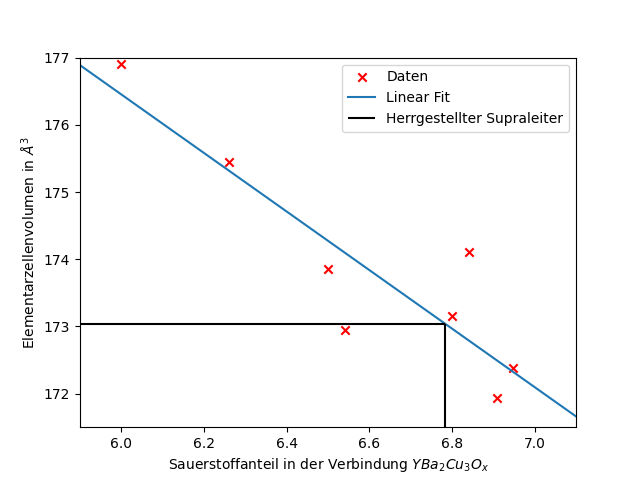
\includegraphics[scale=0.8]{Plot.png}
  \caption{Zeigt das Elementarzellenvolumen gegen den Sauerstoffgehalt mit einen Linearen Fit und den hergestellten \ce{YBa2Cu3O_{7-\delta}}}
  \label{plot}
\end{figure}

Die neuen









\newpage
\section{Zusammenfassung}




\newpage
\section{Literaturverzeichnis}
\printbibliography







\end{document}